\documentclass[tikz,border=10pt]{standalone}
\usetikzlibrary{arrows.meta, positioning, shapes.geometric, shapes.misc, fit, backgrounds, calc, matrix}

\tikzset{
    >=Latex,
    font=\sffamily\large,
    node distance=1.5cm and 3cm,
    dag_result/.style={
        rectangle, 
        draw=green!70!black, 
        fill=green!15, 
        very thick, 
        minimum width=4.5cm, 
        minimum height=1.5cm, 
        text width=5cm,
        align=center
    },
    dag_lemma/.style={
        rounded rectangle, 
        draw=orange!80!black, 
        fill=yellow!20, 
        very thick, 
        minimum width=4.5cm, 
        minimum height=1.5cm, 
        text width=5cm,
        align=center
    },
    dag_model/.style={
        ellipse, 
        draw=blue!70!black, 
        fill=blue!12, 
        very thick, 
        minimum width=4.5cm, 
        minimum height=1.5cm, 
        text width=4.5cm,
        align=center
    },
    dag_unformalized/.style={
        rectangle, 
        draw=gray!60!black, 
        fill=gray!10, 
        very thick, 
        dashed, 
        minimum width=4.5cm, 
        minimum height=1.5cm, 
        text width=5cm,
        align=center
    },
    dag_conditional/.style={
        rectangle, 
        rounded corners,
        draw=orange!80!black, 
        fill=orange!10, 
        very thick, 
        minimum width=4.5cm, 
        minimum height=1.5cm, 
        text width=5cm,
        align=center
    },
    dag_partial/.style={
        rectangle,
        rounded corners,
        draw=yellow!55!black,
        fill=yellow!10,
        very thick,
        dashed,
        minimum width=4.5cm,
        minimum height=1.5cm,
        text width=5cm,
        align=center
    },
    dag_scaffold/.style={
        rectangle,
        draw=gray!55!black,
        fill=white,
        very thick,
        dotted,
        minimum width=4.5cm,
        minimum height=1.5cm,
        text width=5cm,
        align=center
    },
    dag_caveat/.style={
        diamond, 
        draw=red!70!black, 
        fill=red!10, 
        minimum width=4cm, 
        align=center, 
        inner sep=0pt, 
        font=\sffamily\small
    },
    dag_arrow/.style={
        -{Stealth[scale=1.2]}, 
        very thick,
        shorten >=1.5pt,
        shorten <=1.5pt
    },
    dag_dashed_arrow/.style={
        -{Stealth[scale=1.2]}, 
        very thick, 
        dashed,
        shorten >=1.5pt,
        shorten <=1.5pt
    },
    dag_template_legend/.style={
        minimum width=2.6cm,
        minimum height=0.8cm,
        text width=2.45cm,
        inner sep=3pt,
        font=\sffamily\small,
        align=center
    },
    dag_template_note/.style={
        rectangle,
        draw=gray!50,
        fill=gray!5,
        rounded corners,
        text width=13cm,
        align=left,
        font=\sffamily\small,
        inner sep=6pt
    }
}

% Legend Helper
\newcommand{\daglegend}[2]{
    \node[draw, rounded corners, very thick, fit=#1, inner sep=12pt, label=above:\textbf{\Large Legend}] (#2) {};
}


\begin{document}
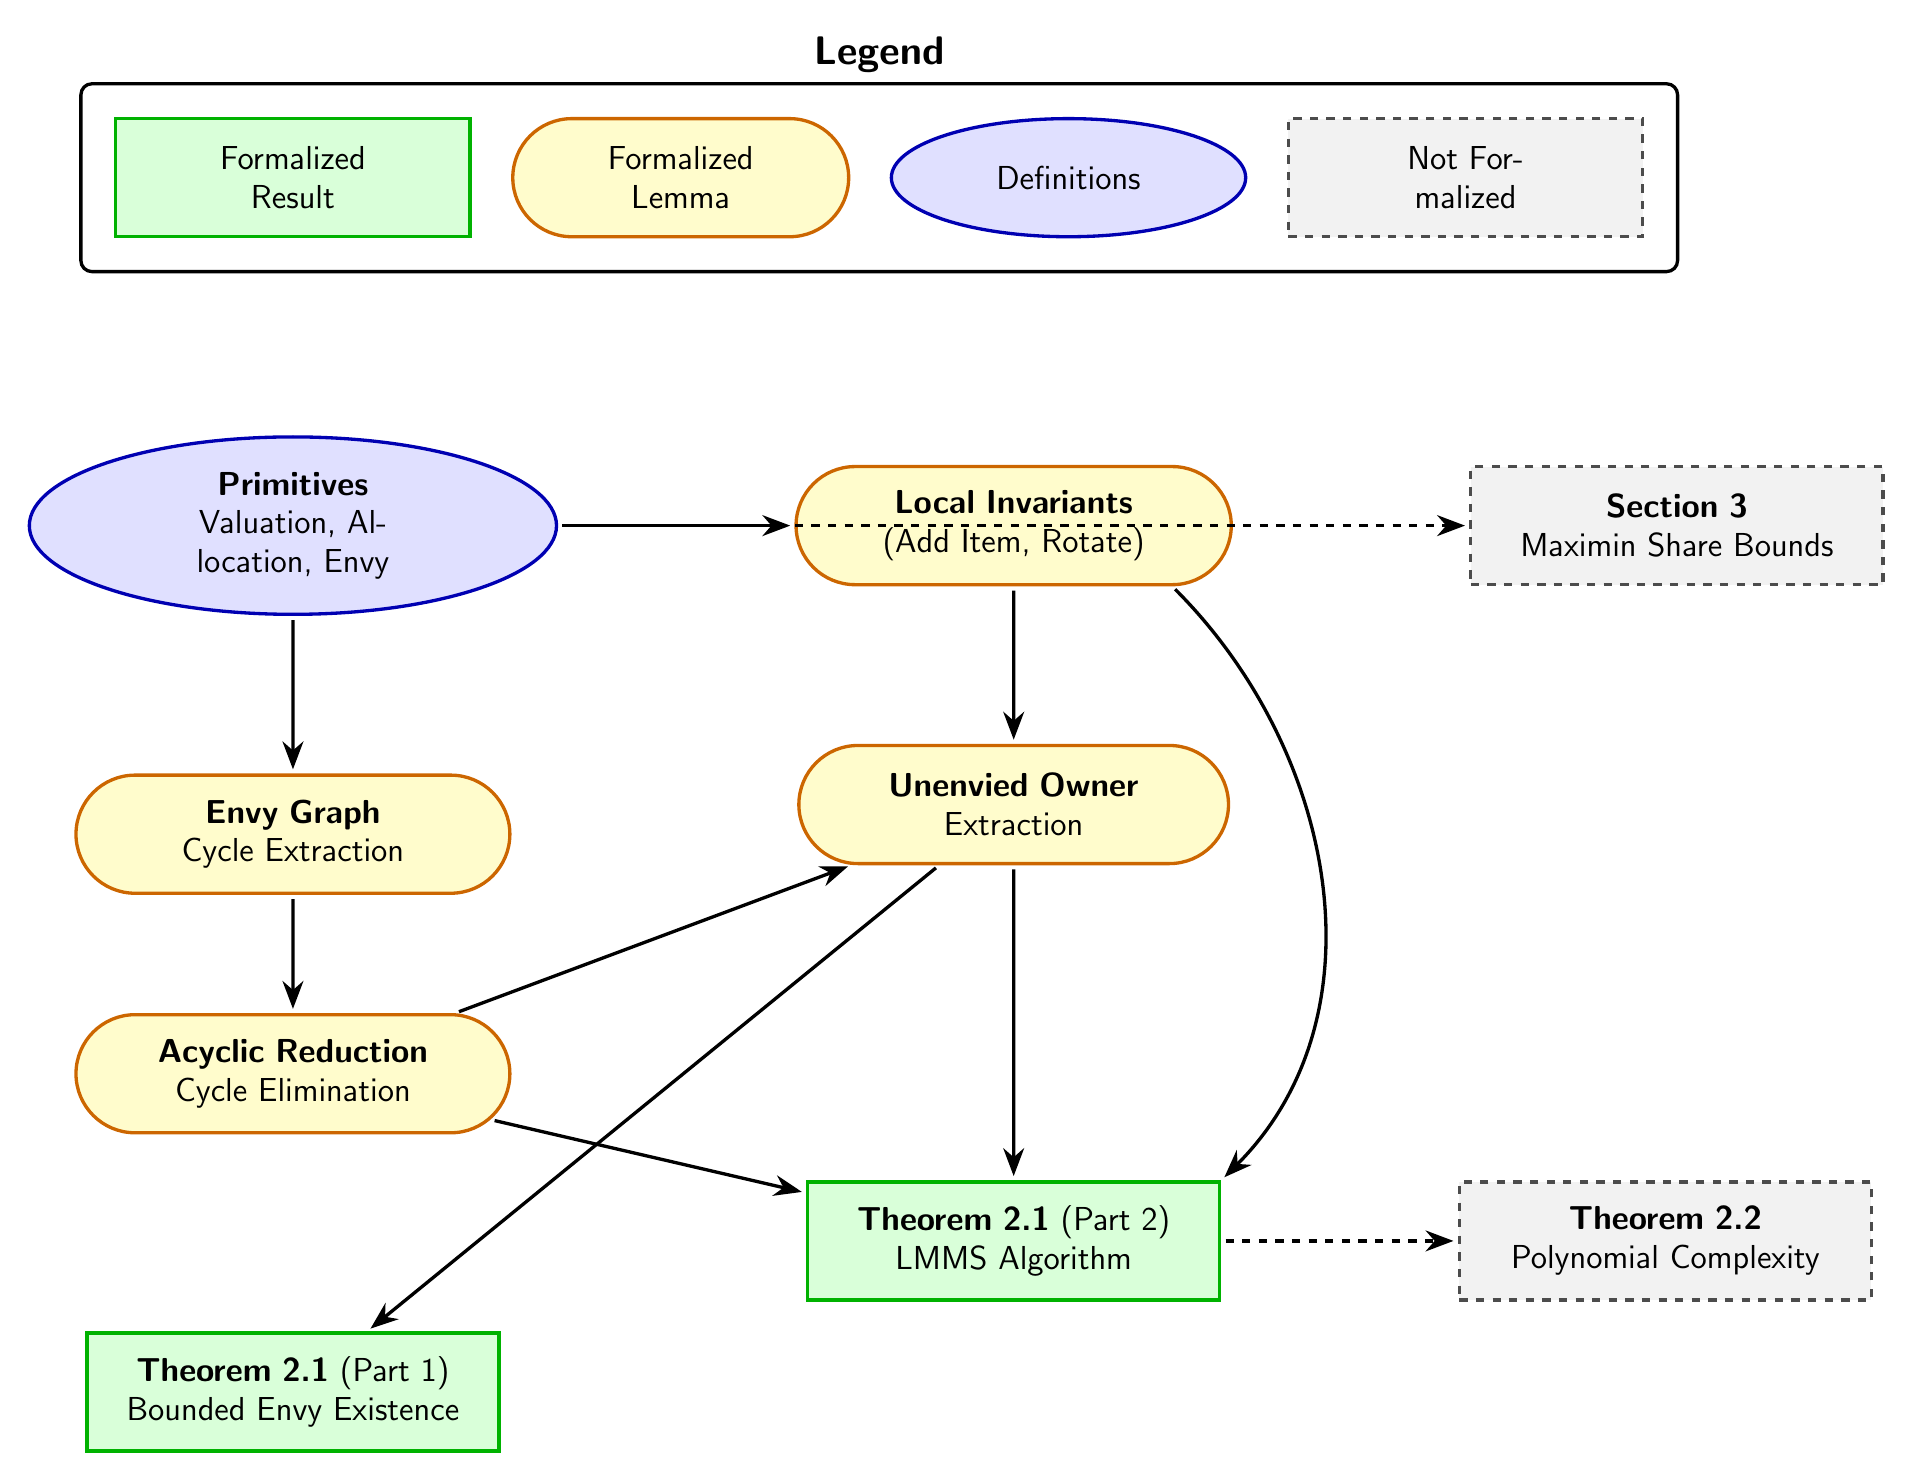
\begin{tikzpicture}

% --- Legend ---
\node[dag_result, text width=2.5cm] (legRes) {Formalized Result};
\node[dag_lemma, right=0.5cm of legRes, text width=2.5cm] (legLem) {Formalized Lemma};
\node[dag_model, right=0.5cm of legLem, text width=2.5cm] (legDef) {Definitions};
\node[dag_unformalized, right=0.5cm of legDef, text width=2.5cm] (legNot) {Not Formalized};
\daglegend{(legRes)(legLem)(legDef)(legNot)}{Legend}

% --- Column 1 (Primitives & Graph) ---
\node[dag_model, below=2.5cm of legRes] (Primitives) {\textbf{Primitives} \\ Valuation, Allocation, Envy};
\node[dag_lemma, below=2cm of Primitives] (Graph) {\textbf{Envy Graph} \\ Cycle Extraction};
\node[dag_lemma, below=1.5cm of Graph] (Acyclic) {\textbf{Acyclic Reduction} \\ Cycle Elimination};
\node[dag_result, below=2.5cm of Acyclic] (ThmExist) {\textbf{Theorem 2.1} (Part 1) \\ Bounded Envy Existence};

% --- Column 2 (Local & Algorithm) ---
\node[dag_lemma, right=of Primitives] (Local) {\textbf{Local Invariants} \\ (Add Item, Rotate)};
\node[dag_lemma, below=2cm of Local] (Unenvied) {\textbf{Unenvied Owner} \\ Extraction};
\node[dag_result, below=4cm of Unenvied] (ThmAlgo) {\textbf{Theorem 2.1} (Part 2) \\ LMMS Algorithm};

% --- Column 3 (Extensions) ---
\node[dag_unformalized, right=of Local] (Sec3) {\textbf{Section 3} \\ Maximin Share Bounds};
\node[dag_unformalized, right=of ThmAlgo] (Thm2_2) {\textbf{Theorem 2.2} \\ Polynomial Complexity};

% --- Edges ---
\draw[dag_arrow] (Primitives) -- (Graph);
\draw[dag_arrow] (Primitives) -- (Local);
\draw[dag_arrow] (Graph) -- (Acyclic);
\draw[dag_arrow] (Local) -- (Unenvied);
\draw[dag_arrow] (Acyclic) -- (Unenvied);
\draw[dag_arrow] (Unenvied) -- (ThmExist);
\draw[dag_arrow] (Unenvied) -- (ThmAlgo);
\draw[dag_arrow] (Local.south east) to[out=315, in=45] (ThmAlgo.north east);
\draw[dag_arrow] (Acyclic) -- (ThmAlgo);

\draw[dag_dashed_arrow] (ThmAlgo) -- (Thm2_2);
\draw[dag_dashed_arrow] (Primitives) -- (Sec3);

\end{tikzpicture}
\end{document}
